% =============================================
% 导言区
% =============================================
\documentclass{xjtureport}








% =============================================
% 正文区
% =============================================


\begin{document}

% ===导入实验报告封面==============================
\begin{titlepage}
	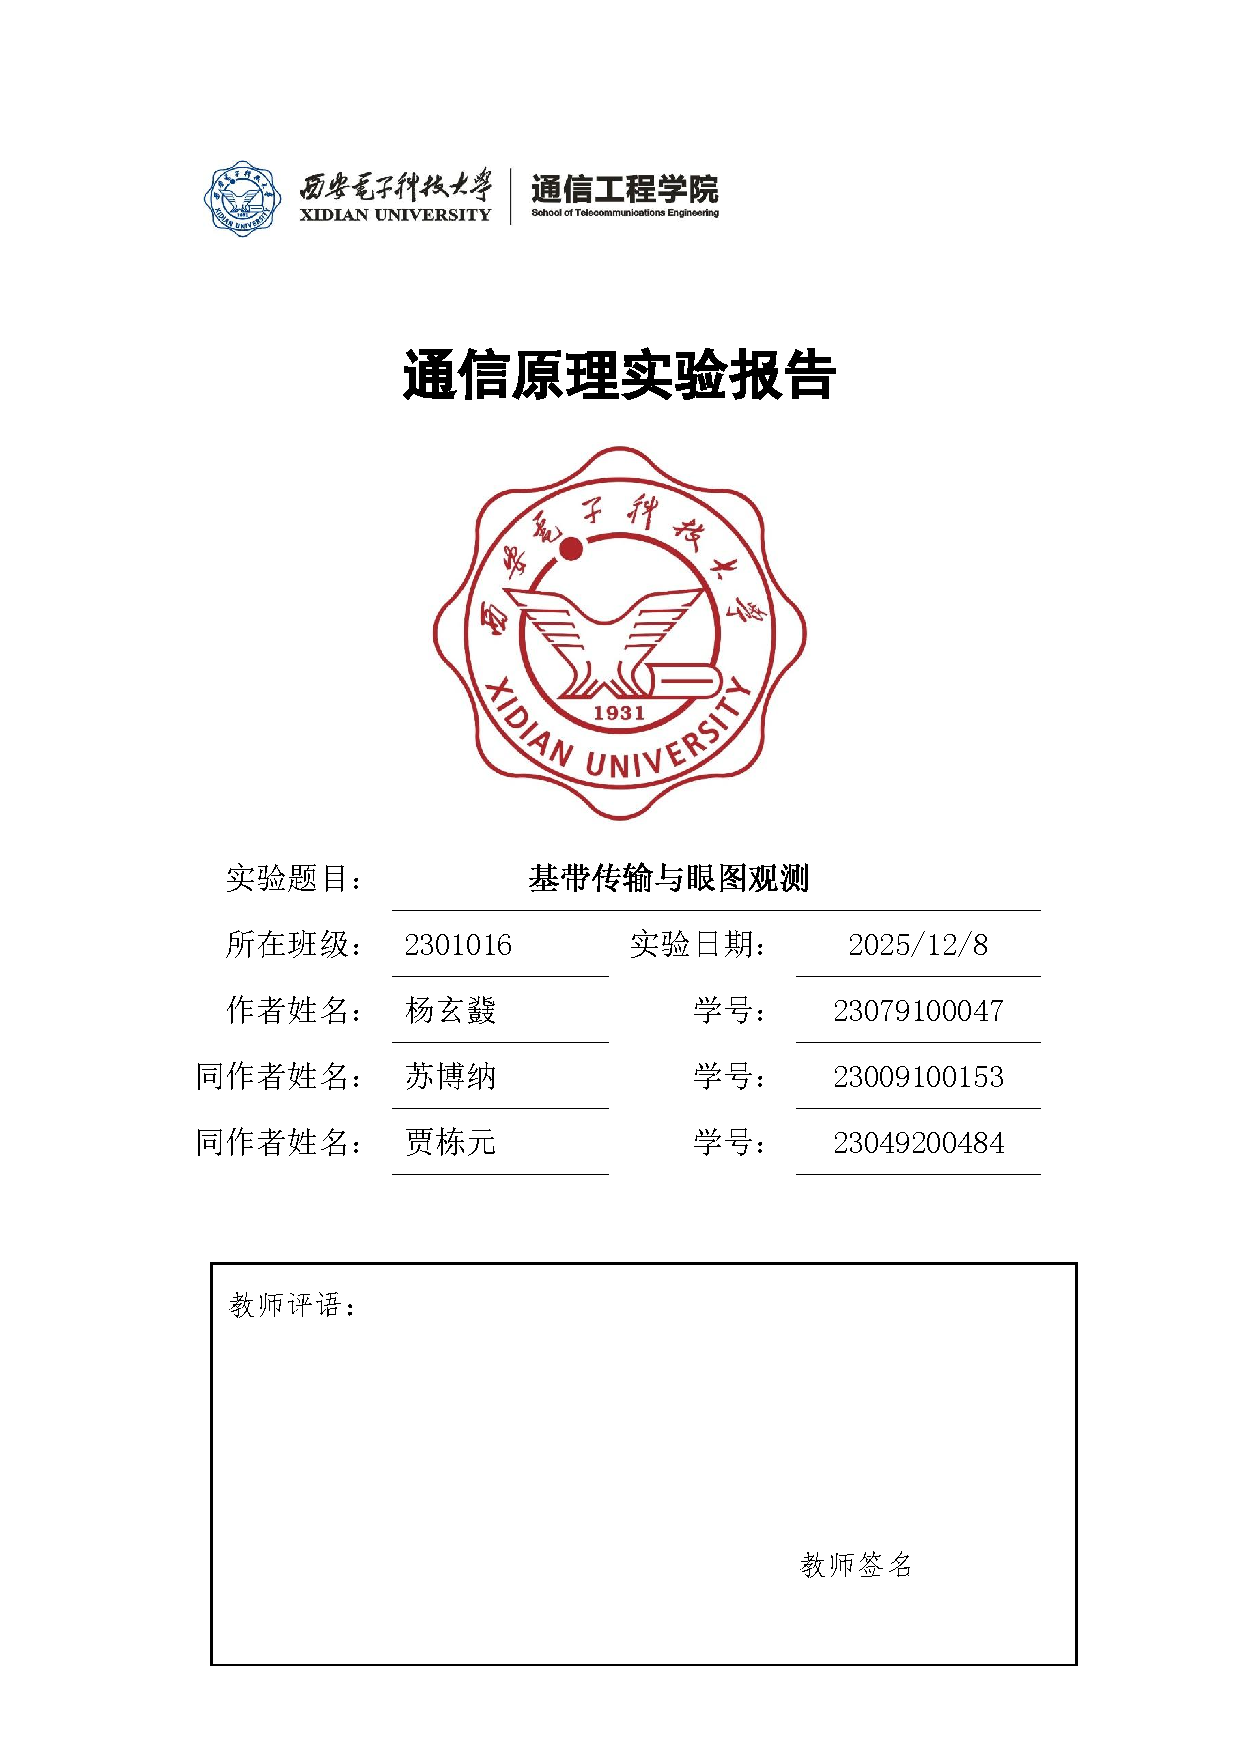
\includepdf[pages=-]{figures/实验5封面.pdf}
\end{titlepage}



% ===正文==============================


% 标题（一级居中）

\chapterinline{实验五： 基带传输与眼图观测实验}

\section{实验目的}
（1）掌握眼图观测方法

（2）学会用眼图分析通信系统性能

\section{实验器材}

西电通信与实验专业平台（半实物仿真）。

\section{实验内容}

\subsection*{(1) 成型信号观测}

将基带信号设置为“511-PN”，“32K”，采用示波器一个通道观测 2P6 端口基带信号，另一通道观测 4VT11 端口成型输出信号。分别选用高斯滤波器、升余弦滤波器和根升余弦滤波器作为成型滤波方式，在时域上对比成型前后的波形变化，并利用示波器 FFT 功能观测对应信号的频谱特性，从而定性比较不同成型方式对信号带宽及频谱分布的影响。

\textbf{实验结果：}

%==================== 高斯滤波 ====================
\begin{figure}[H]
	\centering
	\begin{subfigure}{0.31\linewidth}
		\centering
		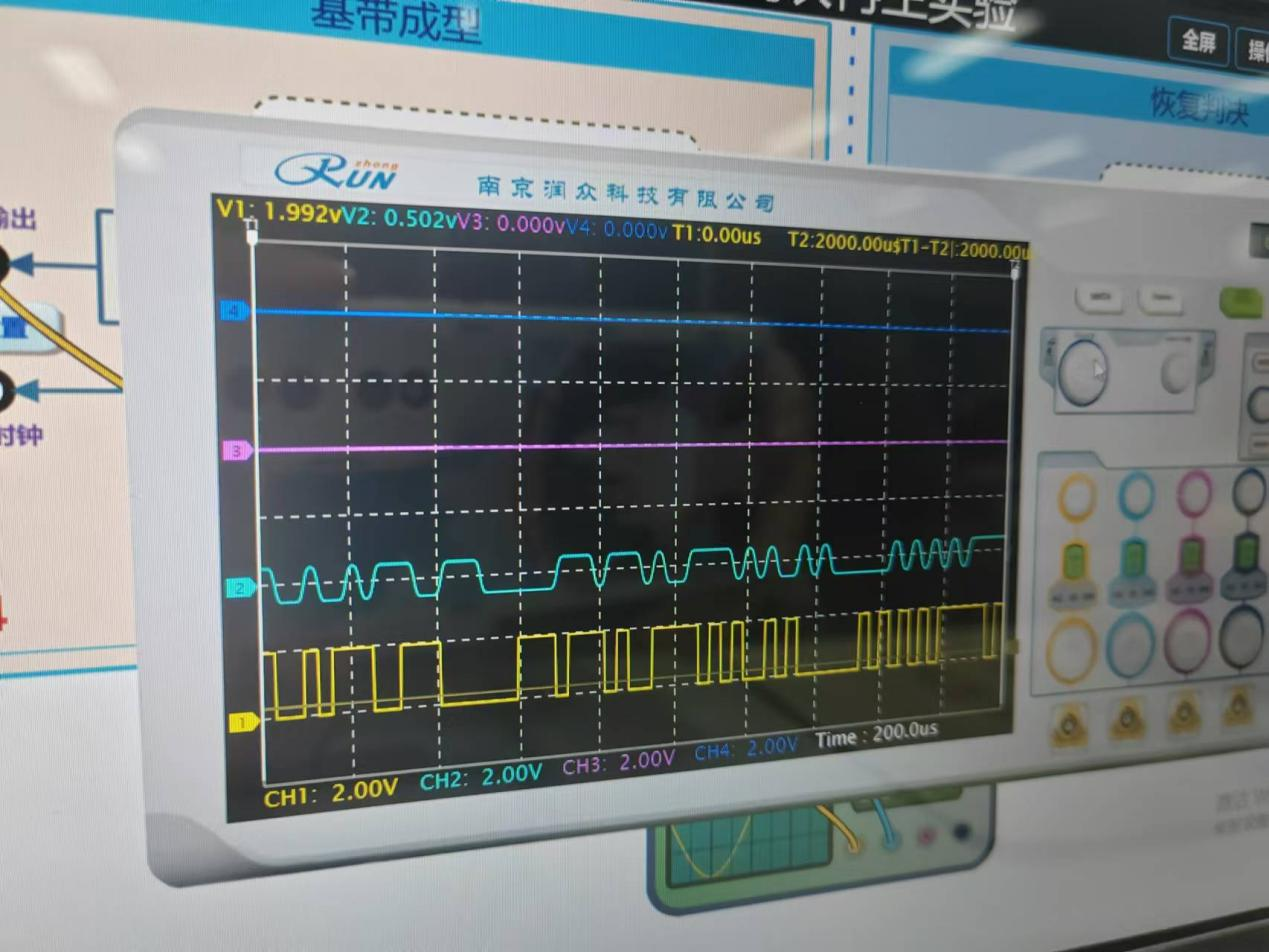
\includegraphics[width=\linewidth]{figures/高斯滤波_成型前后时域信号.png}
		\caption{高斯滤波成型前后时域波形}
	\end{subfigure}
	\hfill
	\begin{subfigure}{0.31\linewidth}
		\centering
		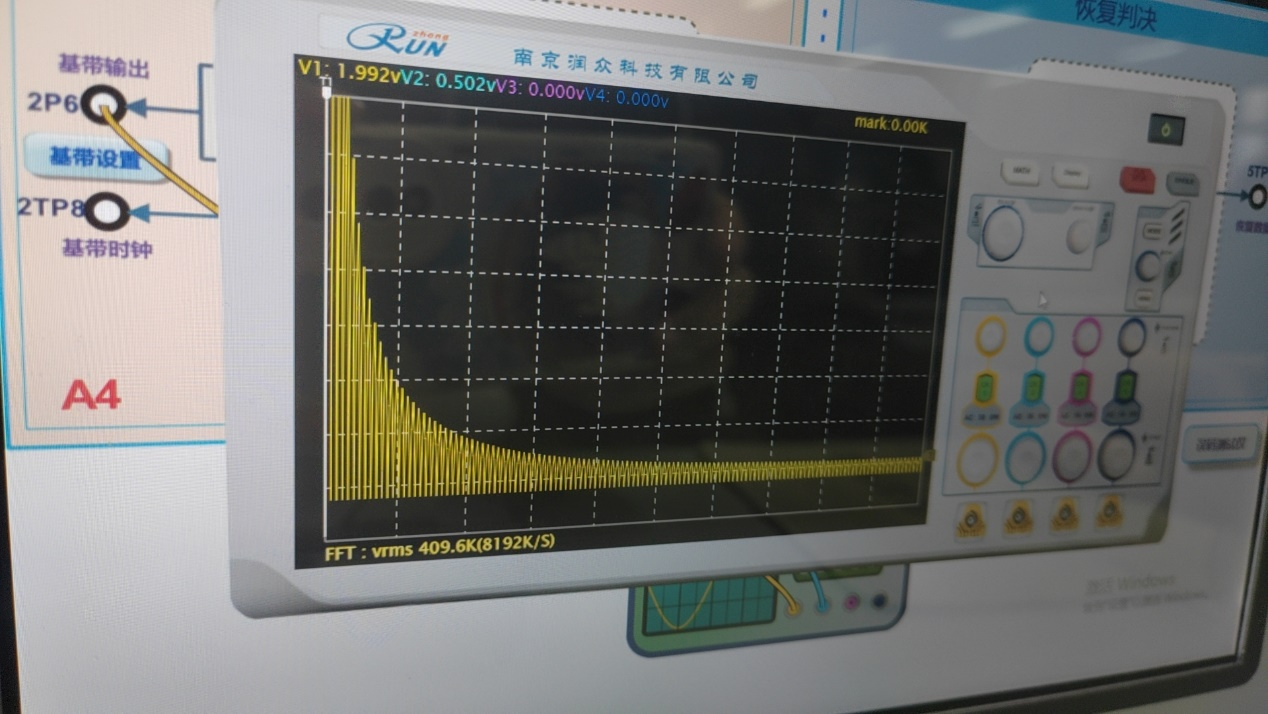
\includegraphics[width=\linewidth]{figures/高斯滤波_成型前信号频谱.png}
		\caption{高斯滤波成型前信号频谱}
	\end{subfigure}
	\hfill
	\begin{subfigure}{0.31\linewidth}
		\centering
		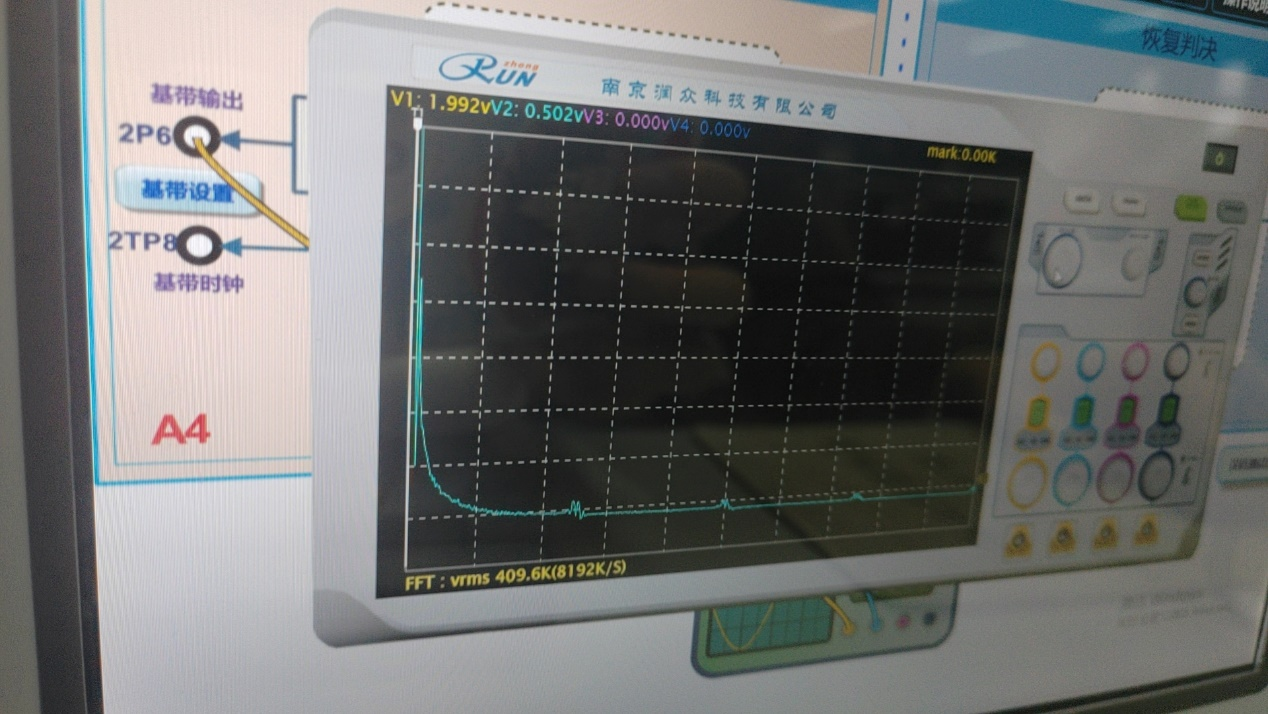
\includegraphics[width=\linewidth]{figures/高斯滤波_成型后信号频谱.png}
		\caption{高斯滤波成型后信号频谱}
	\end{subfigure}
	\caption{高斯滤波成型前后信号的时域与频域特性}
\end{figure}

%==================== 升余弦滤波 ====================
\begin{figure}[H]
	\centering
	\begin{subfigure}{0.32\linewidth}
		\centering
		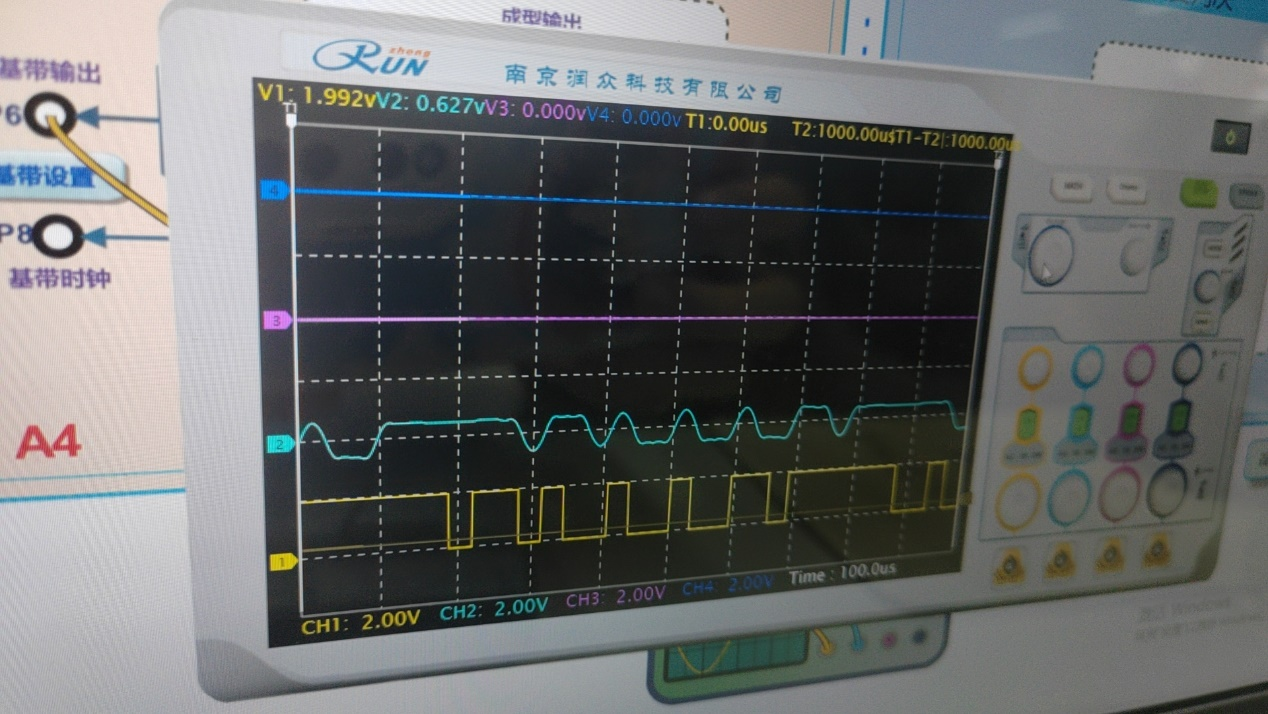
\includegraphics[width=\linewidth]{figures/升余弦滤波_成型前后时域信号.png}
		\caption{升余弦滤波成型前后时域波形}
	\end{subfigure}
	\hfill
	\begin{subfigure}{0.32\linewidth}
		\centering
		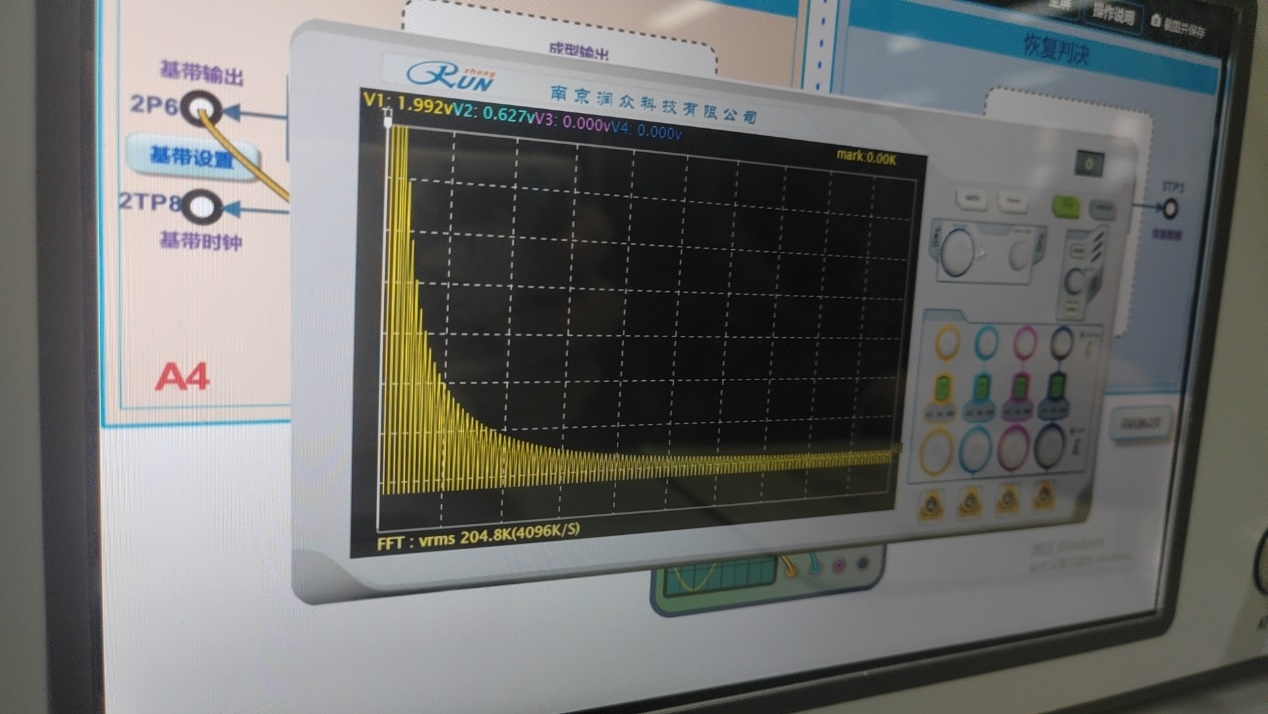
\includegraphics[width=\linewidth]{figures/升余弦滤波_成型前信号频谱.png}
		\caption{升余弦滤波成型前信号频谱}
	\end{subfigure}
	\hfill
	\begin{subfigure}{0.32\linewidth}
		\centering
		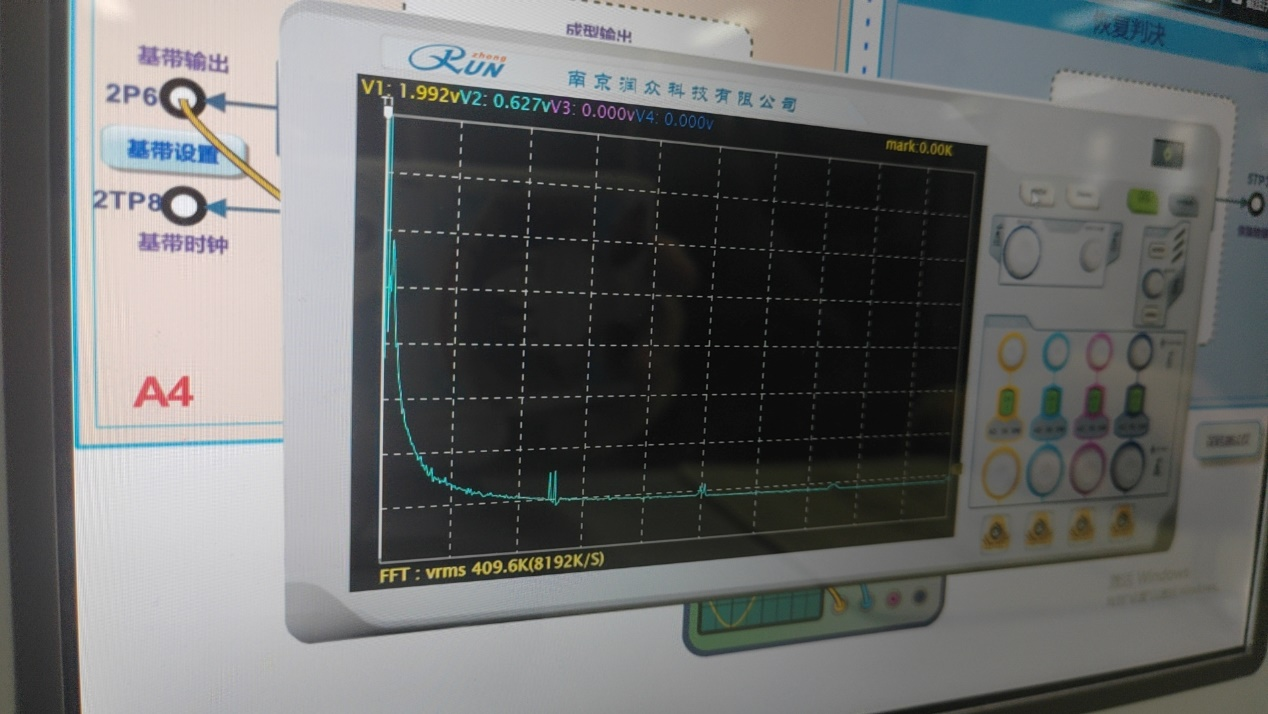
\includegraphics[width=\linewidth]{figures/升余弦滤波_成型后信号频谱.png}
		\caption{升余弦滤波成型后信号频谱}
	\end{subfigure}
	\caption{升余弦滤波成型前后信号的时域与频域特性}
\end{figure}

%==================== 根升余弦滤波 ====================
\begin{figure}[H]
	\centering
	\begin{subfigure}{0.32\linewidth}
		\centering
		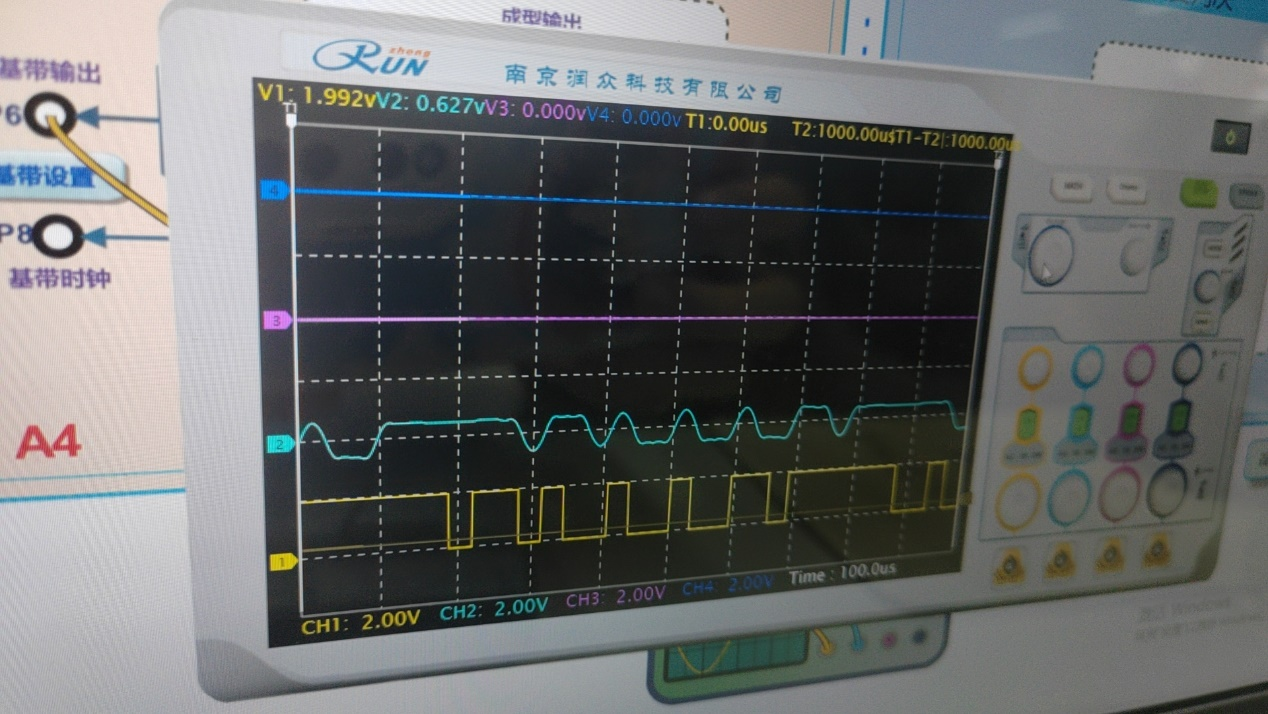
\includegraphics[width=\linewidth]{figures/根升余弦_成型前后时域信号.png}
		\caption{根升余弦滤波成型前后时域波形}
	\end{subfigure}
	\hfill
	\begin{subfigure}{0.32\linewidth}
		\centering
		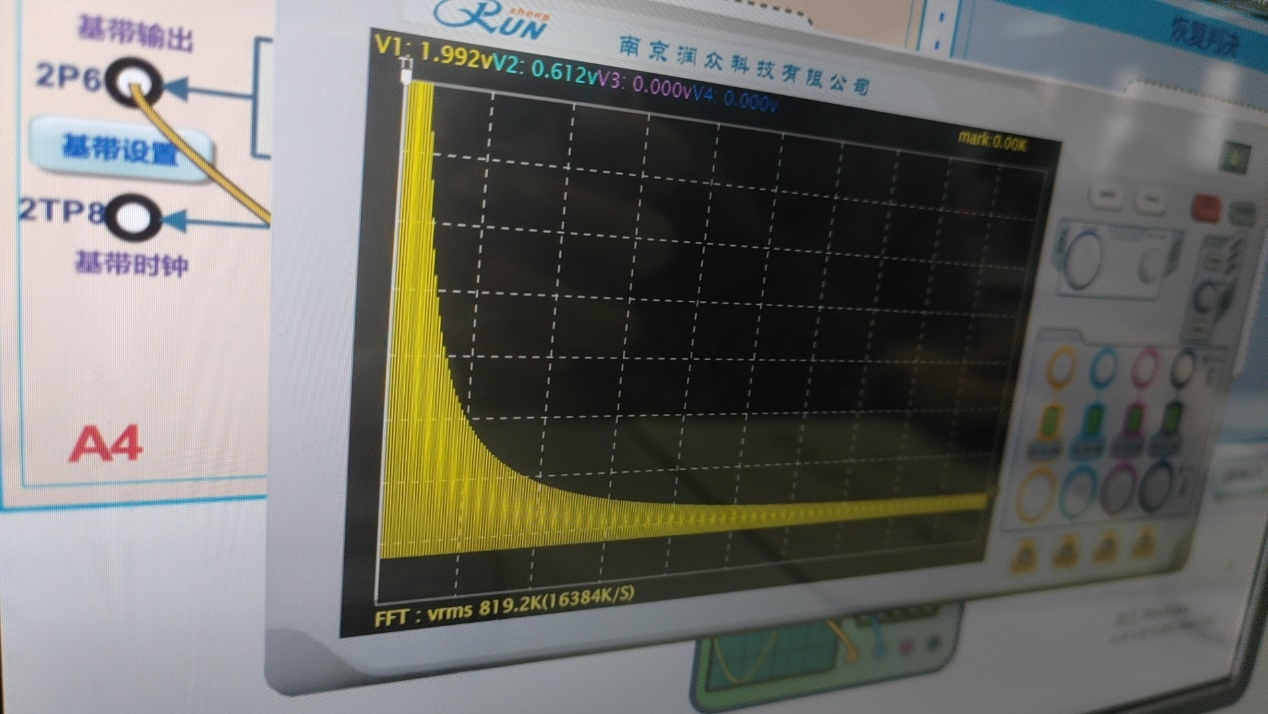
\includegraphics[width=\linewidth]{figures/根升余弦_成型前信号频谱.png}
		\caption{根升余弦滤波成型前信号频谱}
	\end{subfigure}
	\hfill
	\begin{subfigure}{0.32\linewidth}
		\centering
		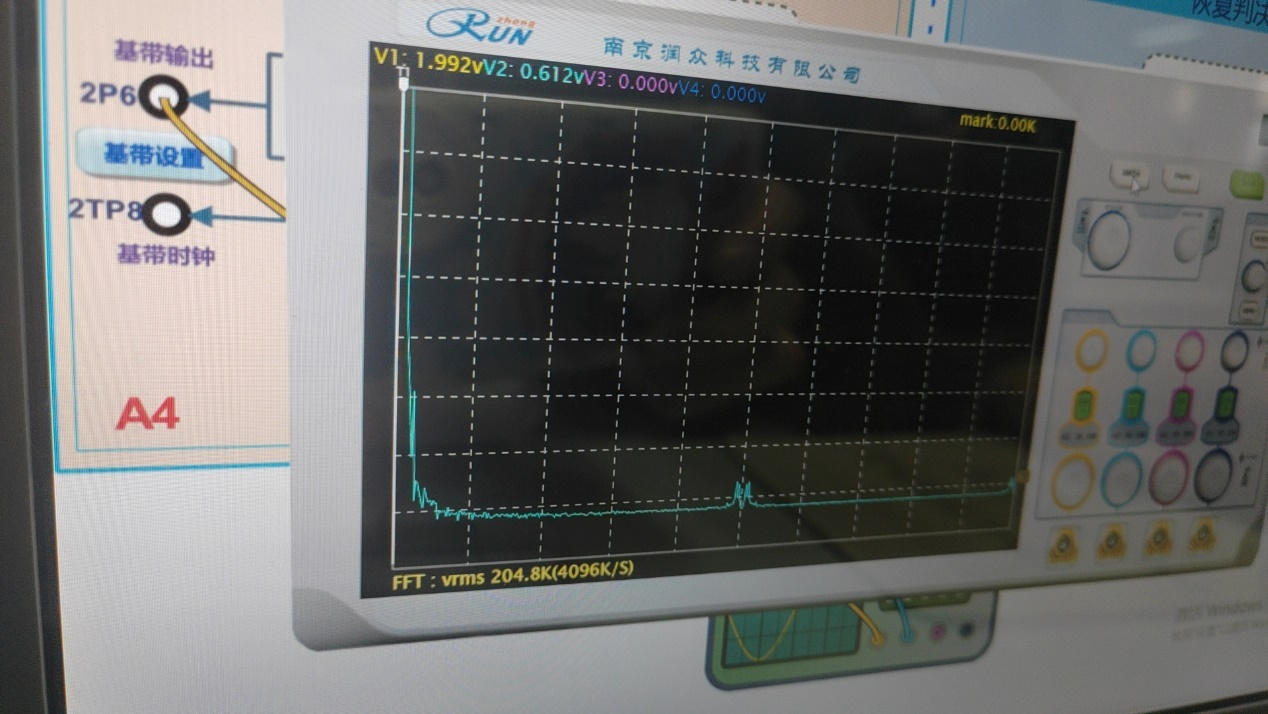
\includegraphics[width=\linewidth]{figures/根升余弦_成型后信号频谱.png}
		\caption{根升余弦滤波成型后信号频谱}
	\end{subfigure}
	\caption{根升余弦滤波成型前后信号的时域与频域特性}
\end{figure}

\textbf{分析：}

由成型信号的时域与频域观测结果可知，未经成型的基带信号在时域上呈现为突变明显的矩形脉冲，其频谱分布较为分散，包含较多高频分量，占用带宽较宽。经过成型滤波后，信号波形趋于平滑，高频分量受到抑制，频谱能量向低频集中，信号的有效带宽明显减小。

对比不同成型方式可见，高斯滤波对高频分量的抑制最为显著，频谱衰减平缓，带宽压缩效果明显；升余弦滤波在频域上具有较为清晰的带宽边界，频谱集中度高，有利于提高频谱利用率；根升余弦滤波在带宽限制与频谱平滑性之间取得折中，其频谱分布介于高斯滤波与升余弦滤波之间。

综上，不同成型滤波器均能够有效限制基带信号带宽，但在频谱分布形态和高频抑制特性方面存在差异，这些差异将直接影响后续基带传输性能。

\subsection*{(2) 无噪声模拟信道眼图观测}

将基带数据设置为“511-PN”，“32K”，在无噪声模拟信道条件下，分别选用高斯滤波、升余弦滤波和根升余弦滤波作为成型方式，利用示波器的眼图显示功能，观测并比较不同成型方式下眼图的张开情况。

\textbf{实验结果：}

\begin{figure}[H]
	\centering
	\begin{subfigure}{0.31\linewidth}
		\centering
		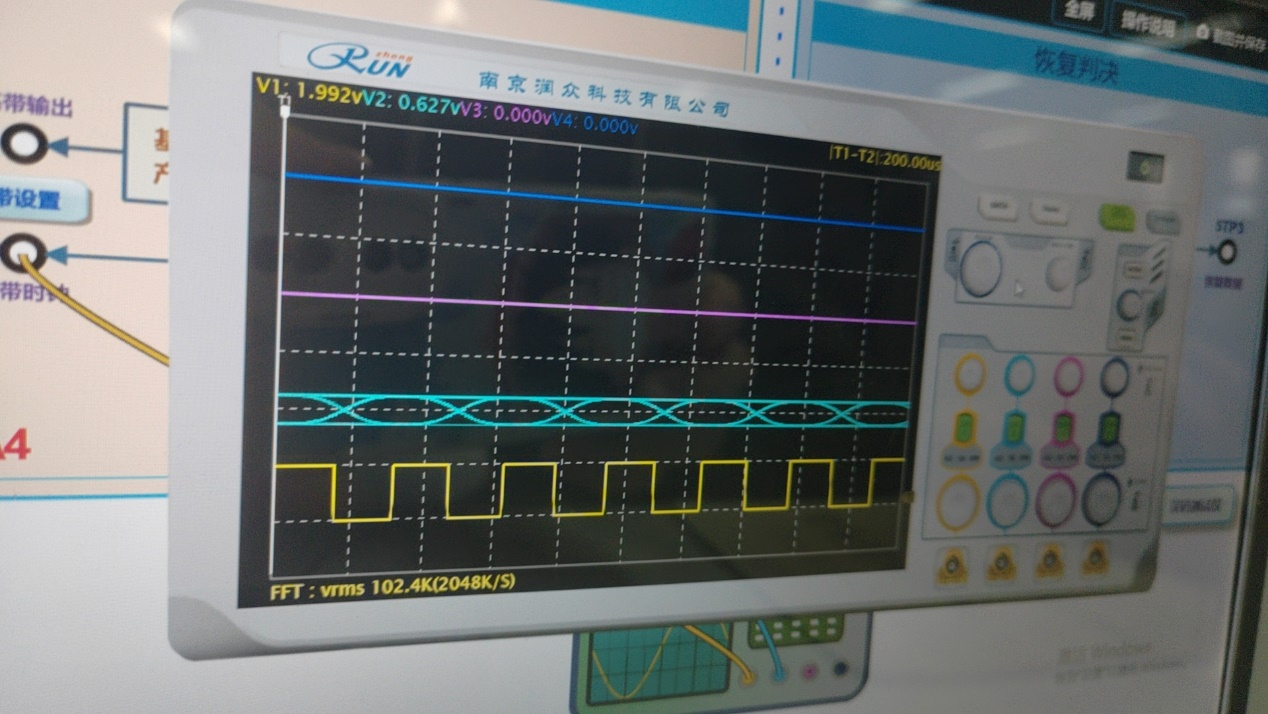
\includegraphics[width=\linewidth]{figures/高斯滤波_无噪声模拟信道眼图.png}
		\caption{高斯滤波成型下的无噪声眼图}
	\end{subfigure}
	\hfill
	\begin{subfigure}{0.31\linewidth}
		\centering
		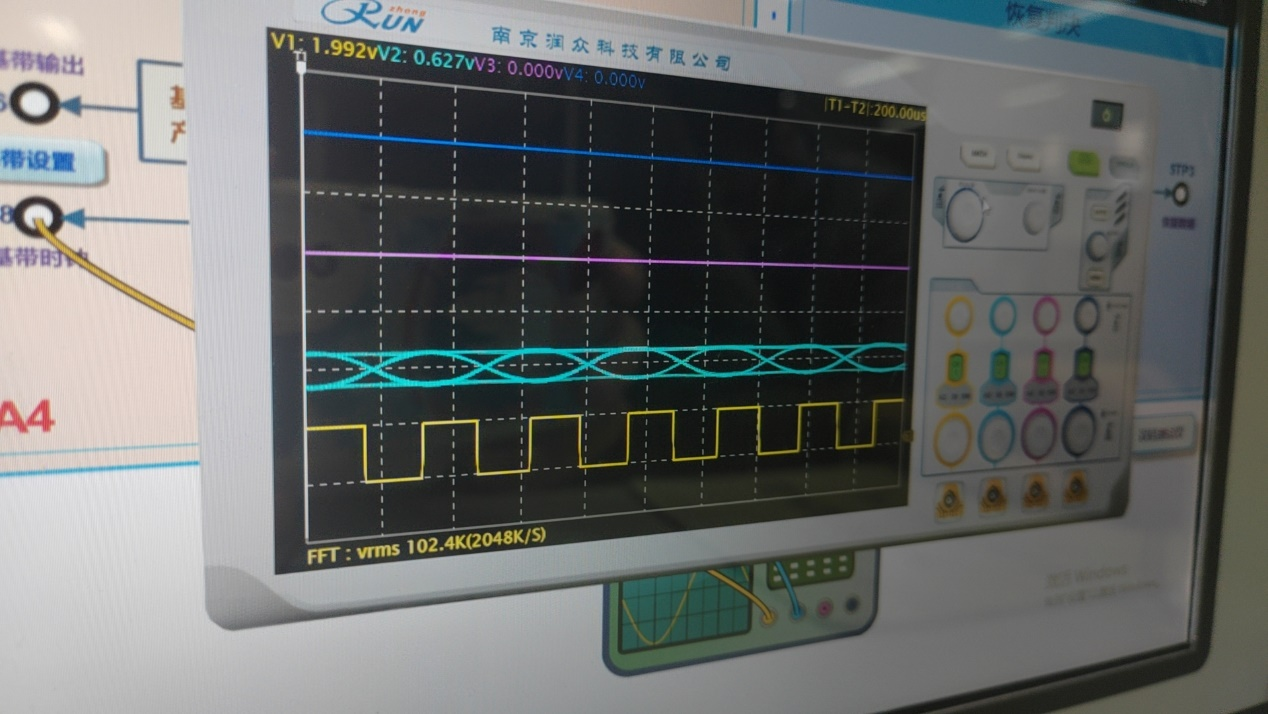
\includegraphics[width=\linewidth]{figures/升余弦_无噪声模拟信道眼图.png}
		\caption{升余弦滤波成型下的无噪声眼图}
	\end{subfigure}
	\hfill
	\begin{subfigure}{0.31\linewidth}
		\centering
		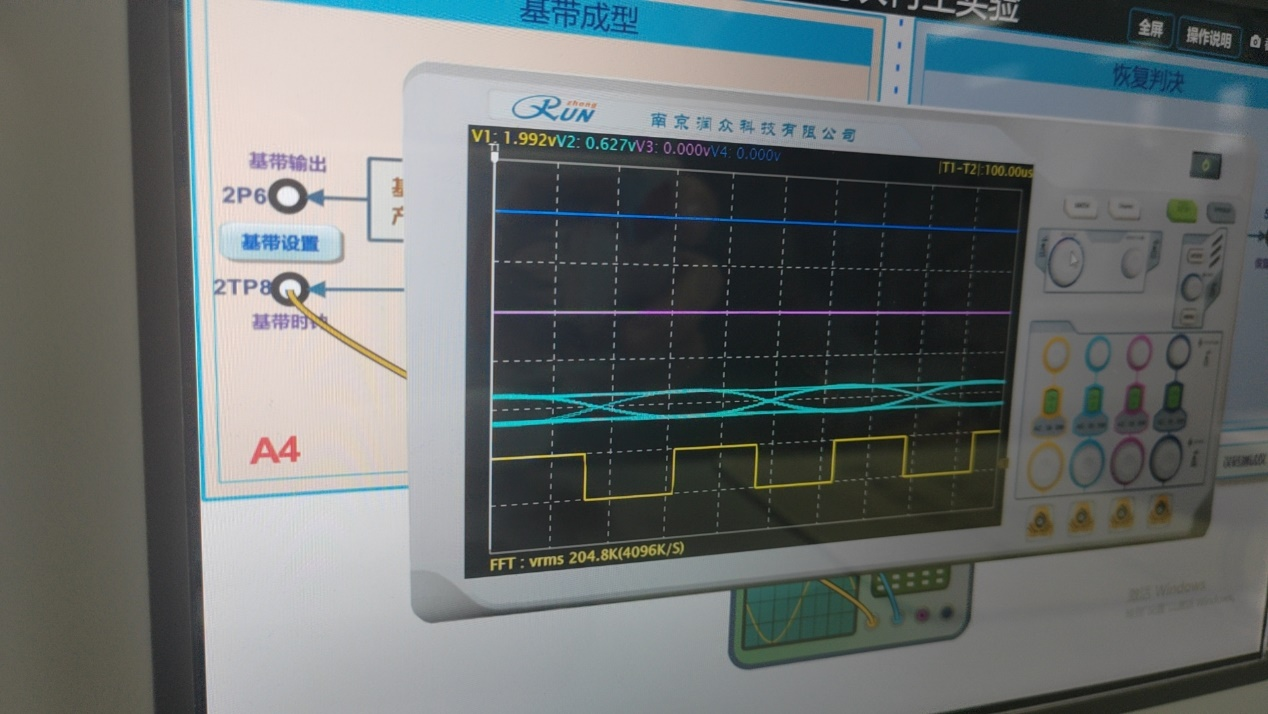
\includegraphics[width=\linewidth]{figures/根升余弦_无噪声模拟信道眼图.png}
		\caption{根升余弦滤波成型的无噪声眼图}
	\end{subfigure}
	\caption{无噪声条件下不同成型方式的眼图对比}
\end{figure}

\textbf{分析：}

在无噪声条件下，眼图的张开程度主要由成型方式决定。由实验结果可见，高斯滤波成型下的眼图在符号过渡区存在一定的重叠，眼口相对较窄，表明码间干扰影响较为明显；升余弦滤波成型下的眼图眼口较为清晰，张开度明显改善；根升余弦滤波成型下的眼图在采样时刻处开口最大，符号间干扰最小。

\subsection*{(3) 有噪声模拟信道眼图观测}

在成型方式保持不变的条件下，引入加性噪声并逐步改变噪声幅度，观察不同噪声强度对接收端眼图形态的影响。实验中选用高斯滤波作为成型方式，噪声幅度分别设置为 20、40 和 60，对应记录三幅眼图并进行比较分析。

\textbf{实验结果：}

\begin{figure}[H]
	\centering
	\begin{subfigure}{0.55\linewidth}
		\centering
		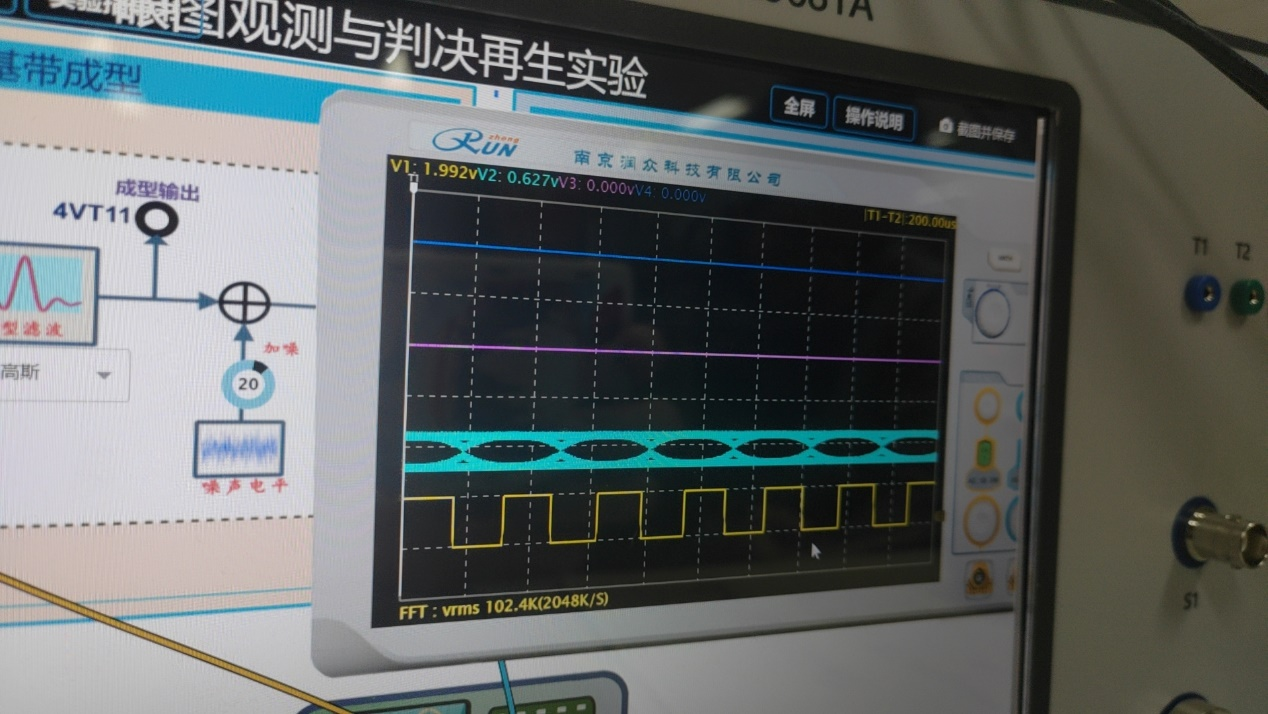
\includegraphics[width=\linewidth]{figures/高斯滤波_有噪声模拟信道眼图_噪声20.png}
		\caption{噪声幅度为 20 时的眼图}
	\end{subfigure}
	
	\vspace{0.6em}
	
	\begin{subfigure}{0.55\linewidth}
		\centering
		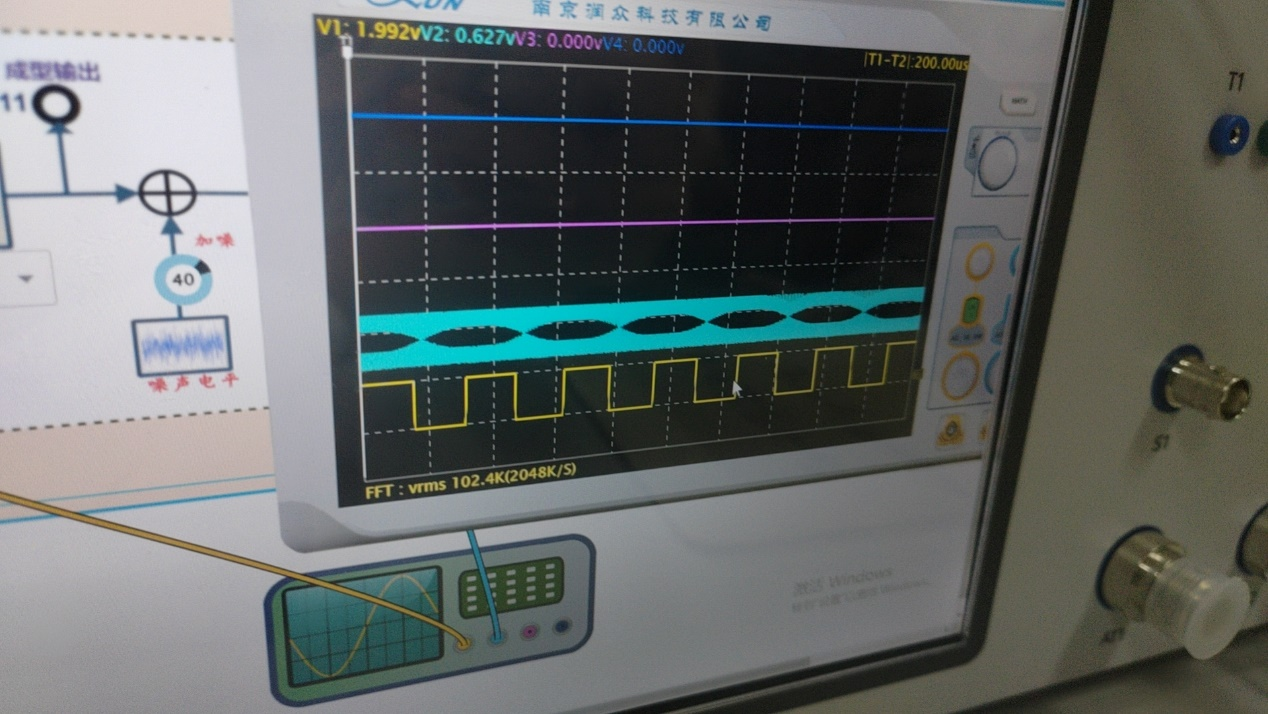
\includegraphics[width=\linewidth]{figures/高斯滤波_有噪声模拟信道眼图_噪声40.png}
		\caption{噪声幅度为 40 时的眼图}
	\end{subfigure}
	
	\vspace{0.6em}
	
	\begin{subfigure}{0.55\linewidth}
		\centering
		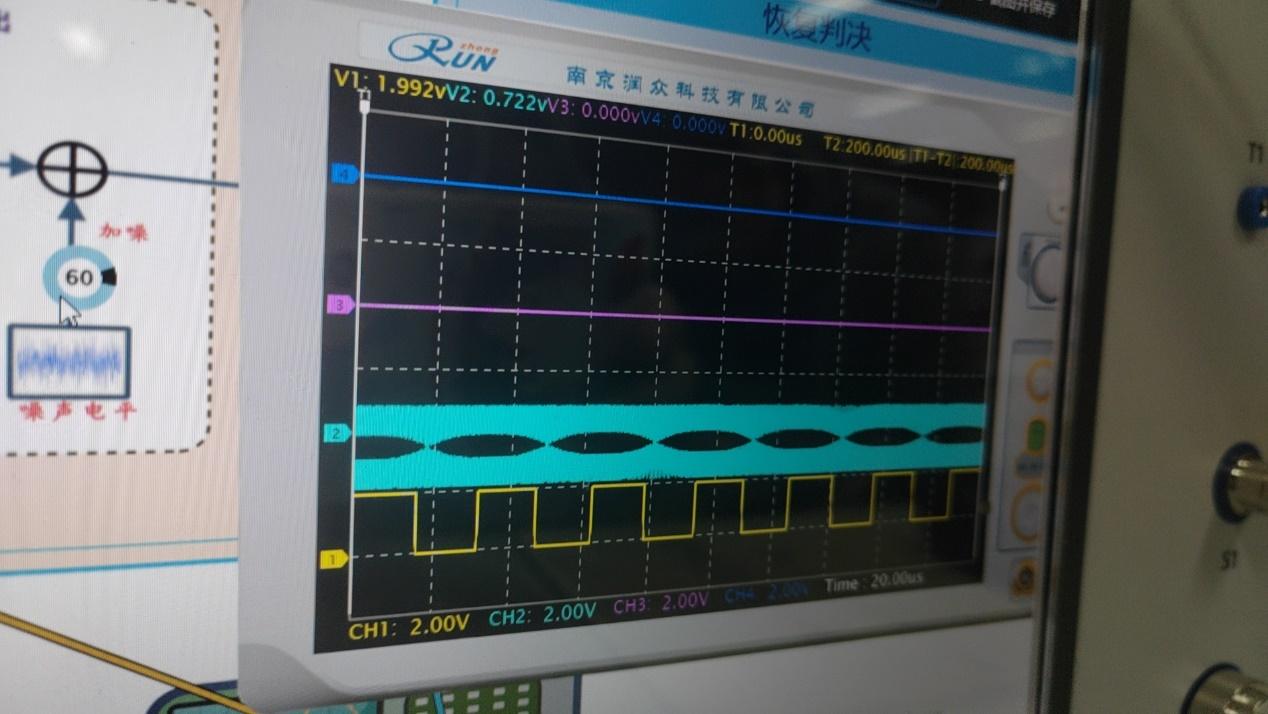
\includegraphics[width=\linewidth]{figures/高斯滤波_有噪声模拟信道眼图_噪声60.png}
		\caption{噪声幅度为 60 时的眼图}
	\end{subfigure}
	\caption{不同噪声幅度下高斯滤波成型信号的眼图}
\end{figure}

\textbf{分析：}

由实验结果可见，随着噪声幅度的逐步增大，眼图的张开程度明显减小。噪声幅度较小时，眼口仍然清晰，符号电平区分较为明显；当噪声幅度增大时，眼图上下边界抖动加剧，眼口高度明显缩小；在噪声幅度较大时，眼图出现明显模糊，采样时刻处的不确定性显著增加。

因此，在有噪声模拟信道中，噪声幅度的增加会直接降低眼图的张开度，加大码元再生时的判决不确定性，从而对系统的可靠传输产生不利影响。



\subsection*{(4) 恢复判决观测}

在无噪声条件下，保持成型方式与基带数据设置不变，通过调节判决电平参数，观测判决电平过低、正常以及过高时恢复判决输出的变化情况，并分析判决电平对码元再生的影响机理。

\textbf{实验结果：}

\begin{figure}[H]
	\centering
	\begin{subfigure}{0.45\linewidth}
		\centering
		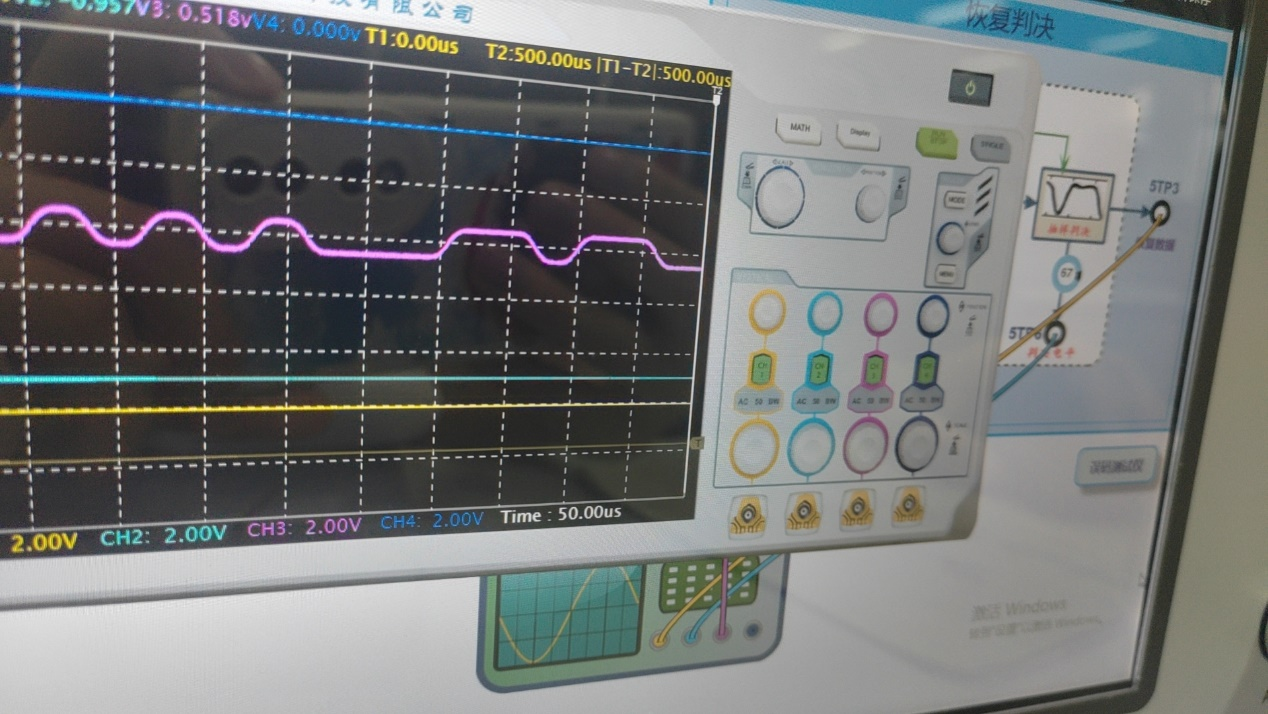
\includegraphics[width=\linewidth]{figures/判决电平过低.png}
		\caption{判决电平过低}
	\end{subfigure}
	\hfill
	\begin{subfigure}{0.45\linewidth}
		\centering
		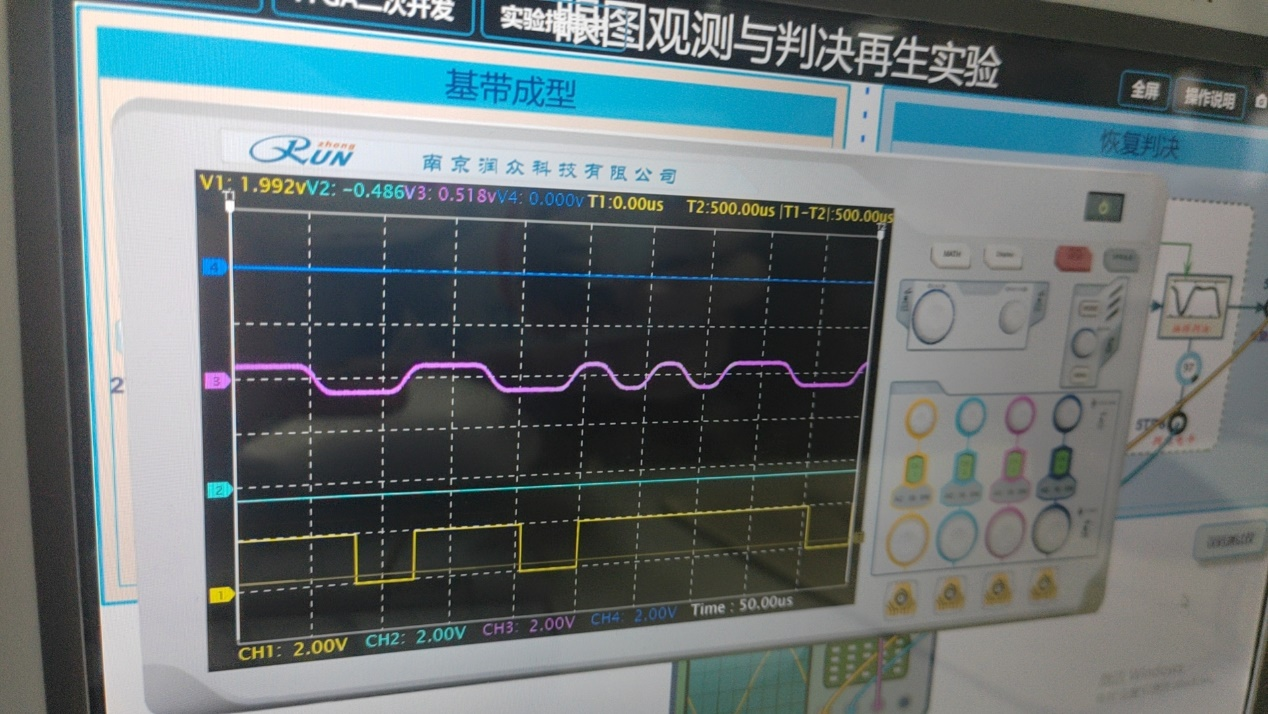
\includegraphics[width=\linewidth]{figures/判决电平过低与正常之间.png}
		\caption{判决电平由低向正常调节}
	\end{subfigure}
	
	\vspace{0.6em}
	
	\begin{subfigure}{0.45\linewidth}
		\centering
		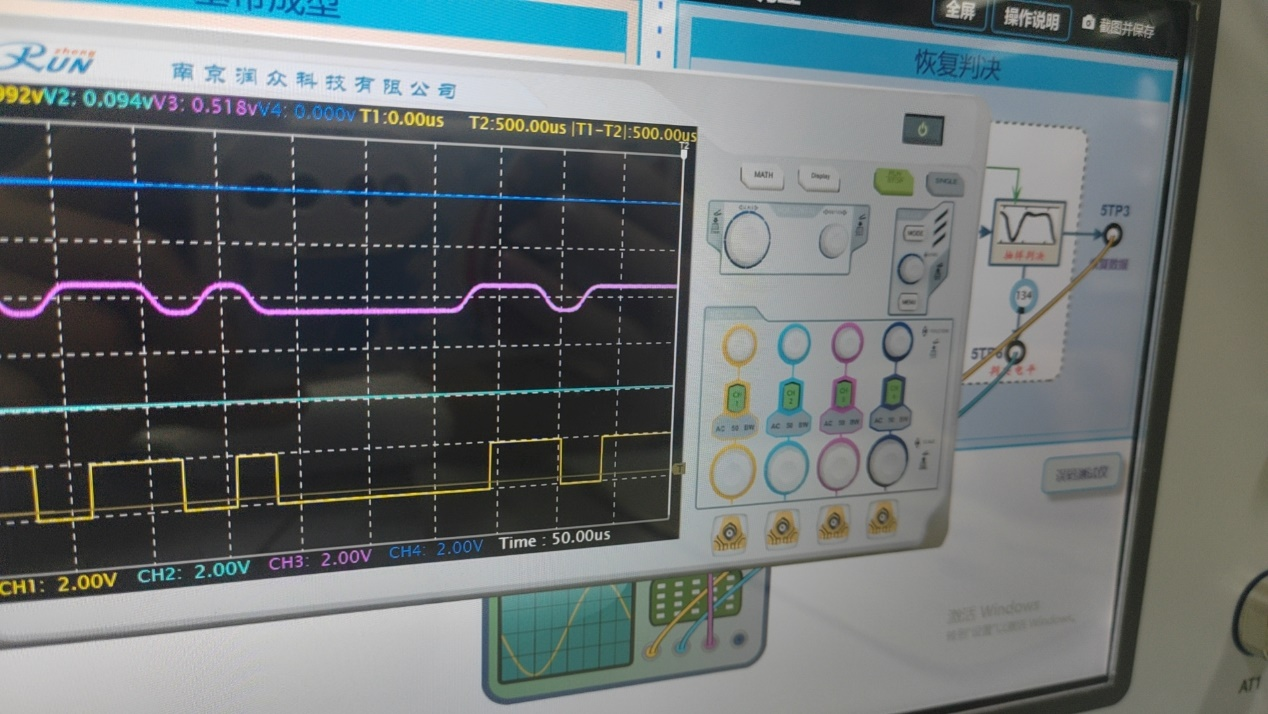
\includegraphics[width=\linewidth]{figures/判决电平正常.png}
		\caption{判决电平正常}
	\end{subfigure}
	\hfill
	\begin{subfigure}{0.45\linewidth}
		\centering
		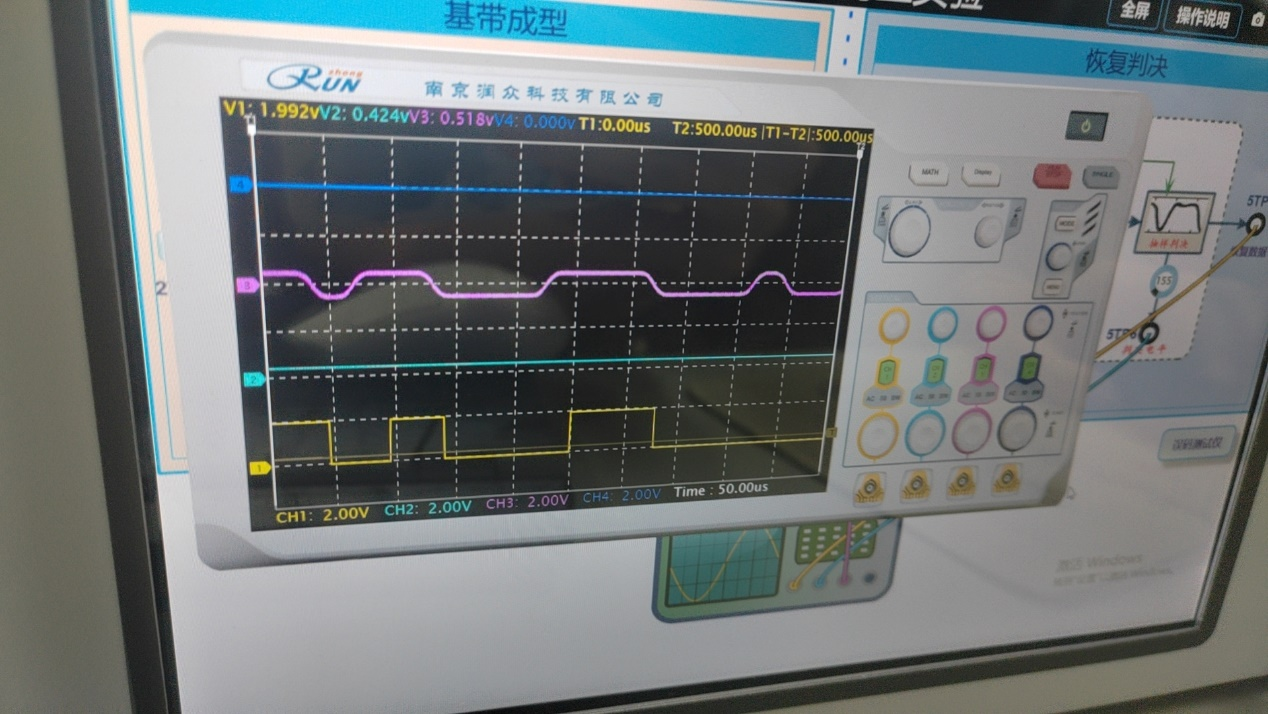
\includegraphics[width=\linewidth]{figures/判决电平过大与正常之间.png}
		\caption{判决电平由正常向高调节}
	\end{subfigure}
	
	\vspace{0.6em}
	
	\begin{subfigure}{0.5\linewidth}
		\centering
		
\includegraphics[width=\linewidth]{figures/判决电平过大.png}
		\caption{判决电平过高}
	\end{subfigure}
	
	\caption{无噪声条件下不同判决电平设置对恢复判决输出的影响}
\end{figure}

\textbf{分析：}

由实验结果可见，判决电平决定了接收信号在采样时刻的电平比较基准，从而直接影响码元的恢复结果。当判决电平设置正常时，恢复判决输出与原始基带数据一致；当判决电平偏低时，较多采样点会被判为“高电平”，导致恢复数据出现偏高（误判增多）；当判决电平偏高时，较多采样点会被判为“低电平”，导致恢复数据出现偏低（误判增多）。因此，判决门限应设置在两种码元电平的合理分界处（通常接近眼图开口中心对应的最佳判决区域），以保证码元再生正确。


\section{问题回答}

\subsection*{1. 眼图的原理是什么？}

\textbf{答：} 眼图是将接收端基带信号按码元周期进行同步截取，并在同一时间窗口内多次叠加显示而形成的波形图。通过这种叠加方式，可以直观反映信号在一个码元周期内的幅度变化情况，从而综合体现码间干扰、噪声以及定时偏差等因素对基带传输性能的影响。

\subsection*{2. 眼图在通信系统中的意义.}

\textbf{答：}
眼图是评价数字通信系统传输性能的重要时域工具。通过观察眼图的张开程度、交叉点位置及边缘模糊程度，可以直观判断码间干扰和噪声对信号的影响，并据此评估系统的抗干扰能力、判决电平选择是否合理以及定时同步的可靠性。


\section{心得体会}

通过本次实验，我系统地观察和比较了不同基带成型方式对信号时域波形、频谱特性以及眼图形态的影响，加深了对成型滤波在限制信号带宽、抑制码间干扰方面作用的理解。实验过程中结合示波器的时域、频域与眼图观测手段，使我对理论中“带宽—波形—误码性能”之间的关系有了更加直观和深入的认识。同时，通过有噪声信道和判决电平调节实验，进一步体会到噪声强度和判决参数对码元恢复性能的重要影响，为后续数字通信系统的分析与设计奠定了实践基础。


\end{document}